

\chapter{Marco Te\'orico}
\label{cap:preliminares}



\section{Fabricación aditiva}

El Estándar Internacional ISO/ASTM 52900 del año 2015 establece y define los términos usados en la tecnología de manufactura aditiva, relativos a la impresión 3D \citep{iso2015}:

\begin{itemize}
\item \textbf{Manufactura aditiva:} proceso de unión de material para producir piezas desde la data de un modelo 3D, usualmente capa sobre capa, que se opone a las metodologías de manufactura sustractiva y formativa.
\item \textbf{Máquina de manufactura aditiva:} sección de n sistema de manufactura aditiva. Incluye hardware, software de control de la máquina, requiere de un software de configuración y accesorios periféricos para completar el ciclo de construcción para producir piezas.
\item \textbf{Usuario de sistema de manufactura aditiva:} Operador o entidad que utiliza por entero un sistema de manufactura aditiva, o cualquier componente del sistemaenvelope aditivo.
\item \textbf{Extrusión de material:} Proceso de manufactura aditiva en el cual el material es dispensado selectivamente a través de un orificio de una boquilla. 
\item \textbf{Impresora 3D:} Fabricación de objetos a través de la deposición de material usando un cabezal de impresión, boquilla u otra tecnología de impresión.
\item \textbf{Ciclo de construcción:}  Proceso de ciclo simple en el cual uno o más componentes son construidos por capas en la cámara de procesos de un sistema de manufactura aditiva.
\item \textbf{Plataforma de construcción:} (de una máquina) base que provee una superficie sobre la cual son construidas las piezas, desde el inicio y a través de todo el proceso de construcción.
\item \textbf{Capas: } material dispuesto o extendido para crear una superficie.
\item \textbf{Envoltura de construcción:} dimensiones máximas externas de los ejes-x, -y , y eje-z dentro del espacio de construcción donde las piezas pueden ser fabricadas.
\item \textbf{Espacio de construcción:} lugar donde es posible fabricar las piezas, típicamente dentro de la cámara de construcción o sobre la plataforma de construcción.
\item \textbf{Volumen de construcción:} volumen utilizable total, disponible en la máquina para construir piezas.
\item \textbf{Origen, punto cero, (0,0,0):} punto universal de referencia designado, donde los tres ejes de coordenadas primarios se intersectan. 
\item \textbf{Parámetros del proceso:} configuración de los parámetros de operación y ajustes del sistema utilizados durante el ciclo de construcción.
\end{itemize}

\pagebreak

\section{Impresión 3D}

A diferencia de las técnicas principales que se emplean desde hace décadas en la fabricación de objetos, que se encargan de sustraer, combinar, o deformar paulatina y controladamente materia hasta llegar a una pieza final, la impresión 3D funciona de un modo completamente distinto. La pieza se crea en un solo paso, capa por capa, a un ritmo medio de uno a dos centímetro de altura por hora; el objeto creado puede constar de mecanismos internos (como rodamientos de bolas), formas tejidas y entrelazadas, o incluso huecos y curvas \citep{Berchon2014}. Pues bien, todas las impresoras 3D, están basadas sobre el mismo principio: un modelo digital es transformado a un objeto físico de 3 dimensiones por adición de material en capas. Esto se conoce alternativamente como \textit{Manufactura Aditiva} \citep{tresdhub2018}. Este tipo de fabricación también se puede englobar dentro de lo que se denomina \textit{Fabricación digital}, cuyo principio básico es la transformación de la información  desde el mundo físico al digital. Según \citep{jorquera2016}, la fabricación digital incluye los siguientes sistemas y tecnologías:\\
 
 \begin{enumerate}
 	
	\item Sistemas integrados: Es un \textit{hardware} electrónico diseñado específicamente para llevar a cabo una o pocas tareas definidas. Las impresoras llevan un sistema electrónico integrado que utilizan para controlar los motores paso a paso que alimentan el papel, recibir información de los sensores de temperatura y finales de carrera, o que mandan al cabezal de impresión.
	\item Sistemas CNC (\textit{Computer Numeric Control} - control numérico computarizado): Es el control numérico de un sistema de automatización que se utiliza para controlar diferentes máquinas herramienta. Este sistema ha revolucionado la industria gracias a la simplificación del \textit{software} de diseño en conjunto con los lenguajes de programación como el \textit{.gcode}. Esencialmente, un sistema CNC es cualquier sistema que utiliza un ordenador para controlar los movimientos de una máquina.
	\item Software CAD (\textit{Computer Aided Design}- diseño asistido por computador): es, en esencia, un programa que sirve para la creación, edición análisis y visualización de modelos tridimensionales.  
	\item Internet: Los programas CAD actuales disponen de herramientas de trabajo colaborativo en red, de esta manera se define el producto y el proceso de fabricación de forma simultánea.\\

  \end{enumerate}

En la misma línea, y dependiendo de la profundidad técnica que el proceso de fabricación necesite, se agregan los sistemas \citep{leao2017}:

\begin{enumerate}
	\item Software CAE (\textit{Computer Aided Engineering} - Ingeniería Asistida por computador): Son los programas mayoritariamente usados para las tareas de análisis de ingeniería. Estos \textit{softwares}, a través de métodos numéricos como el método de elementos finitos o dinámica de fluidos computacional, se utilizan para, por ejemplo, analizar la robustez y el funcionamiento de ensambles de piezas.
	\item Software CAM (\textit{Computer Aided Manufacturing}- Manufactura Asistida por computador): Corresponde a programas que controlan las herramientas de máquinas de control numérico relacionadas con el proceso de manufactura a realizar, generando un código específico para el producto a fabricar. 

\end{enumerate}



\subsection{Historia de la impresión 3D}

La primera vez que se hizo pública la conceptualización de algo que pudiese parecerse a una impresora 3D, se remonta al año 1964, cuando el científico y escritor británico Arthur C. Clarke realiza la descripción de una máquina ficticia llamada \textit{El Replicador}. En teoría, este artefacto -que en palabras del autor \textit{es la invención que va a poner fin todas las invenciones}- sería capaz de crear una copia exacta de una cosa, reorganizando partículas subatómicas, y luego ensamblar esas moléculas para ser transformadas en un objeto real \citep{renstrom2012}. No obstante, el comienzo de la generación del concepto técnico de impresión 3D puede ser rastreado al año 1976, a partir de la creación de la primera impresora a tinta por inyección \citep{maxey2013}. La utilización de la inyección de tinta abrió la pregunta respecto a qué tipo de materias primas podían ser utilizadas con esta tecnología, y cómo los mecanismos presentes en la época podían ser adaptados para abrir la posibilidad de ocupar otras materias primas. En Mayo de 1981, el Dr. Hideo Kodama del Instituto de Investigación Industrial del Municipio de Nagoya publicó detalles relativos a la técnica de prototipado rápido. Esta investigación se considera como la primera publicación que describe la técnica de fabricación capa a capa propia de los procesos de impresión 3D; no obstante, los desarrollos de Kodama no llegaron a ser materializados debido a problemas encontrados en el proceso de fundido de material. \citep{tresdsourced2020}. Paralelamente, la idea de \textit{máquinas de prototipado rápido} continuó su desarrollo en Francia, por Jean-Claude André, Oliver de Witte y Alain le Méhauté. En la primera mitad de la década de los 80, le Méhauté investigaba en la empresa Alcatel sobre partes y piezas generadas a partir de la geometría fractal, y la manera en que éstas podrían ser fabricadas dada su complejidad de forma.
De Witte, quien era también investigador de Alcatel en el área de luz láser, propuso a le Méhauté que algunos líquidos compuestos por ciertos monómeros podían ser curados y transformados en sólidos tras la aplicación de luz láser, convirtiéndose en el primer paso para la construcción efectiva de máquinas de prototipado rápido a través de el proceso de Estereolitografía. Ambos compartieron el resultado de sus avances con André, que en ese tiempo trabajaba en el Centro Nacional Francés de Investigación Científica, para ya el año 1984 inscribir la patente de su desarrollo. Infortunadamente, el grupo debe abandonar el proyecto debido a problemas con la solidificación del material y poca rentabilidad desde la perspectiva económica \citep{alltresdp2018}.\

Con solo tres semanas de diferencia respecto a los investigadores franceses, Charles Hull, ingeniero graduado de la Universidad de Colorado, solicita la patente del proceso de Esterolitografía con nuevos avances, como la utilización del formato STL (Standard Triangle Language) y la laminación digital de objetos. A diferencia de la Esterolitografía francesa, el método de Hull utiliza luz ultravioleta para el curado de fotopolímeros. El año 1986, obtenida su patente, Hull forma la empresa \textit{3D Systems} y lanza la primera impresora 3D, la \textit{SLA-1}, el año 1987 \citep{tresdsourced2020}. Casi al mismo tiempo, la tecnología de modelado por deposición fundida (FDM) era patentada por Scott Crump como otra tecnología de fabricación aditiva\citep{alltresdp2018}. FDM utiliza un cabezal móvil, el cual funde un filamento de material qie se deposita en una plataforma. Es interesante mencionar que tanto las máquinas SLA como FDM son actualmente las más utilizadas y diversificadas en el mundo de la impresión 3D.
Un año después de la presentación de la SLA-1, Carl Deckard de la Universidad de Texas patentó la tecnología de Sinterizado Selectivo por Láser (SLS). En lugar de utilizar luz ultravioleta, SLS hace uso de un láser para trazar y solidificar las capas de un polvo de polímeros \citep{tresdsourced2020}. Así, la máquina de Deckard se convirtió en la primera impresora 3D en utilizar la tecnología SLS, a la cual llamó Betsy; sin embargo, el propósito central de su invención era testear el sistema de sinterizado por láser, por lo que la calidad de impresión y el nivel de detalle no estaba dentro de sus prioridades\citep{alltresdp2018}. 
En 1993, el MIT desarrolla una técnica de impresión 3D basada en las impresoras de inyección de tinta. Adaptando ésta a un movimiento en un nuevo eje, se crea la Z Corp Z402. El primero modelo utilizaba polvos basados en yeso como base y un aglutinante basado en agua. El mismo año, Royden Sanders fundó Solidscape, creando una impresora 3D basada en cera.
La segunda mitad de los años noventa vio la diversificación de las tecnologías para la técnica de fabricación aditiva, ampliando la gama de materias primas a utilizar y los proceso de transformación de materiales. En 1997, se crea la impresora 3D de metales, la cual utiliza el proceso de fundición por haz de electrones (EBM) y el perfeccionamiento del Polyjet. Así, este desarrollo trajo consigo mayores oportunidades comerciales para estas máquina abriéndose, entre otras, a la industria médica con la bioimpresión de partes adaptables al cuerpo humano tales como piezas dentales o prótesis\citep{tresdsourced2020}.
Los avances de las investigaciones y la búsqueda de la competitividad en la utilización de la impresión 3D como  manufactura aditiva trajo consigo durante los años posteriores el comienzo de la democratización de esta tecnología. Como se ha mostrado en esta sección, la impresión 3D es una tecnología que nace en los años ochenta, por lo cual es factible preguntar cómo y por qué estas máquinas son tan conocidas y valoradas en la actualidad, y de qué manera comienzan a gestar una de las mayores revoluciones tecnológicas del siglo XXI. El proyecto \textit{RepRap} nace el año 2005 a través de un blog impulsado por el doctor Adrian Bowyer, profesor de ingeniería mecánica de la Universidad de Bath del Reino Unido. En él, Bowyer comienza a modelar el primer boceto de una impresora 3D FDM con el objetivo de crear una máquina autoreplicante, capaz de imprimir nuevos componentes en 3D para ser útil en el desarrollo del prototipado rápido, y al mismo tiempo fabricar nuevas piezas para nuevas máquinas. Así, cualquier persona al otro lado del mundo y con las instrucciones adecuadas podría llegar a construirla  \citep{torre2013}. Según Torre (2013) a casi tres años del primer modelo, la \textit{RepRap 0.1} ya había impreso casi la mitad de sus propios componentes; al año 2008, se estima que ya existían más de 100 copias construidas y funcionando en todo el mundo. RepRap es un diseño abierto, y toda la propiedad intelectual producida en este proyecto está sujeto a una licencia de software libre \citep{alltresdp2016}. A partir de esta invención libre, y sumado al vencimiento de las patentes de las tecnologías SLA y FDM, se desata el desarrollo de nuevas impresoras como las de tipología Delta (no cartesiana), y la creación de empresas dedicadas a la fabricación de máquinas de bajo costo como MakerBot \citep{tresdsourced2020}. En la actualidad, se estima que el tamaño del mercado es de alrededor de 10 billones de dólares, y se espera que crezca alrededor de un 23,5\% anualmente, abarcando industrias como la automovilística, aeroespacial, médica, e inclusive el calzado deportivo\citep{donovan2019}.

\begin{figure}[H]
\centering
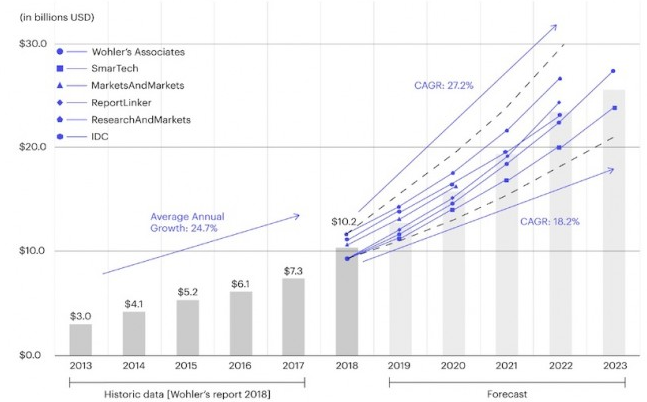
\includegraphics[scale=0.8]{images/3dmarket.png}
\caption{Tamaño del mercado y pronóstico de la impresión 3D \citep{donovan2019}.}

\end{figure}

Respecto al Hype Cycle o ciclo de sobreexpectación de Gartner, el cual corresponde a una publicación anual que representa gráficamente la madurez, adopción y aplicación comercial de tecnologías disruptivas, el inicio del ciclo se caracteriza por usos técnicos especializados como la bioimpresión de órganos, impresión 3D a nanoescala o lo macro fabricación. El peak de expectativas se alcanza con la impresión 3D en el retail para luego decaer en usos pedagógicos o la cadena de suministros. La meseta de productividad se caracteriza por la creación de empresas dedicadas a la impresión 3D, nuevos materiales, la creación de software y servicios. Por otra parte, las predicciones para el año 2019 se centran en el comienzo de la impresión 4D, el auge del sector médico y la impresión 3D de nuevas aleaciones de metal \citep{valdivieso2019}.

\begin{figure}[H]
\centering
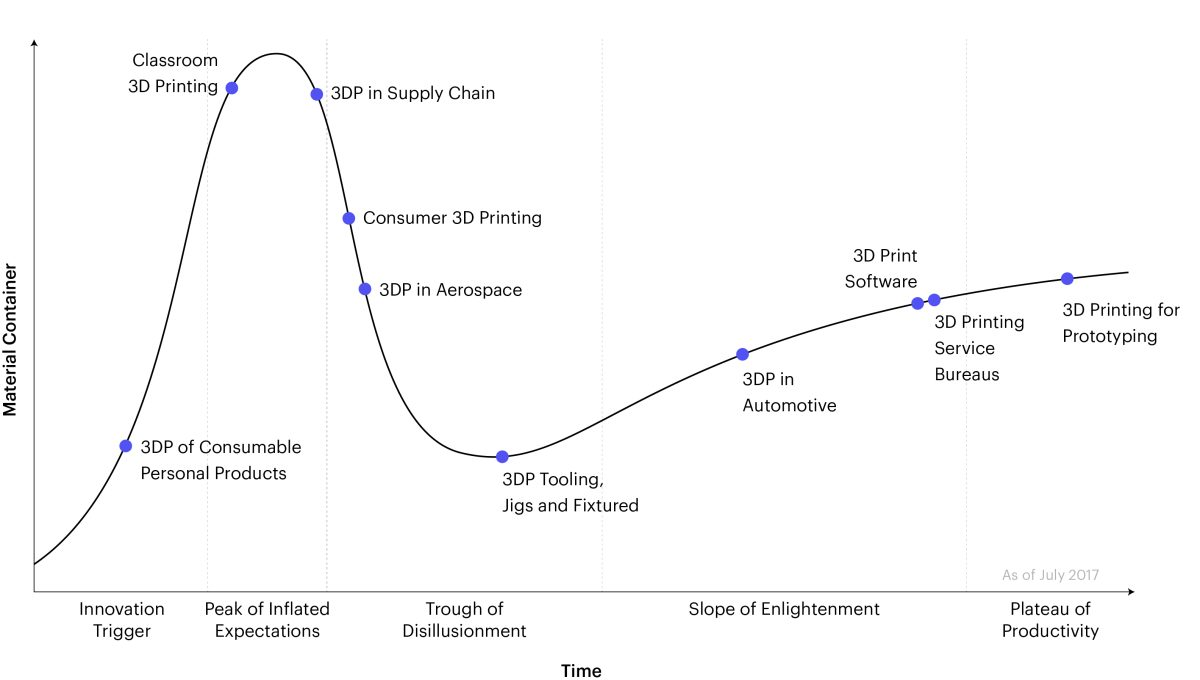
\includegraphics[scale=0.8]{images/The3Dprintinghypecycle.png}
\caption{Hype Cycle o Ciclo de sobreexplotación de Gartner de la tecnología de impresión 3D al año 2019 \citep{valdivieso2019}.}
\end{figure}
  

\subsection{Tecnologías de impresión 3D}

Según la norma ASTM F2792-12a del año 2013 que define el estándar de terminologías para tecnologías de manufactura aditiva, establece las siguientes categorías \citep{astm2013}:

\begin{itemize}
\item \textbf{Chorro de aglutinante:} proceso de manufactura aditiva en el cual un agente líquido de unión es depositado selectivamente para unir polvo de materiales.
\item \textbf{Deposición de energía directa:} proceso de manufactura aditiva en el cual se enfoca energía térmica, que es usada para fundir materiales soldándose a medida que se depositan (láser, flujo de electrones, o arco de plasma).
\item \textbf{Extrusión de material:} proceso de manufactura aditiva en el cual un material es depositado selectivamente a través del orificio de una boquilla.
\item \textbf{Chorro de material:} proceso de manufactura aditiva en el cual gotas del material de construcción son depositadas selectivamente (ejemplo de materiales incluyen fotopolímeros y ceras).
\item \textbf{Fusión de lecho de polvos:} proceso de manufactura aditiva en el cual energía térmica funde selectivamente fusiona regiones del lecho de polvos.
\item \textbf{Laminación:} proceso de manufactura aditiva en el cual láminas de material son depositadas para formar un objeto.
\item \textbf{Fotopolimerización:} proceso de manufactura aditiva en el cual un fotopolímero líquido dentro de un recipiente es curado selectivamente por polimerización de luz activa.
\end{itemize}


\subsection{Impresoras 3D FDM}

Según la norma ASTM F2792-12a, el método de modelado por deposición fundida (FDM por sus siglas en inglés), se define como un proceso de extrusión de material usado para hacer piezas de termoplásticos a través de la extrusión en caliente y la deposición de material capa a capa. Este término denota a las máquinas construidas por la compañía Stratasys \citep{astm2013}. De una forma más amplia, el proceso físico del modelo de fabricación corresponde a un filamento que pasa a través de un elemento calentador, el cual lo convierte en un material fundido o semi-fundido. El filamento ya licuado, es alimentado por una boquilla y depositado sobre la pieza parcialmente construida. El nuevo material añadido se une con el material adyacente ya depositado. El cabezal de extrusión se mueve en el plano X-Y, y vierte controladamente el material acorde a la geometría de las capas ya impresas. Luego de terminar una capa, la plataforma de construcción realiza un movimiento relativo en el eje Z, para comenzar a depositar una nueva capa en la parte superior de la capa anterior. Luego de un tiempo que depende del volumen de la pieza impresa, el cabezal de extrusión habrá realizado una representación física completa del archivo CAD \citep{pdudek2013}.

\begin{figure}[h]
\centering
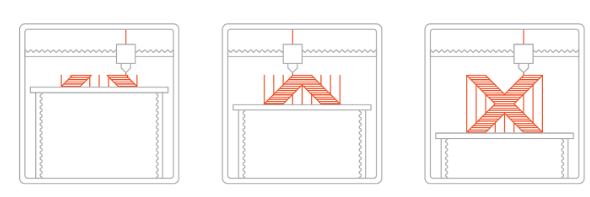
\includegraphics[scale=0.8]{images/fdmprocess.png}
\caption{Proceso de impresión 3D FDM \citep{bournias2017} }
\end{figure}

\begin{figure}[H]
\centering
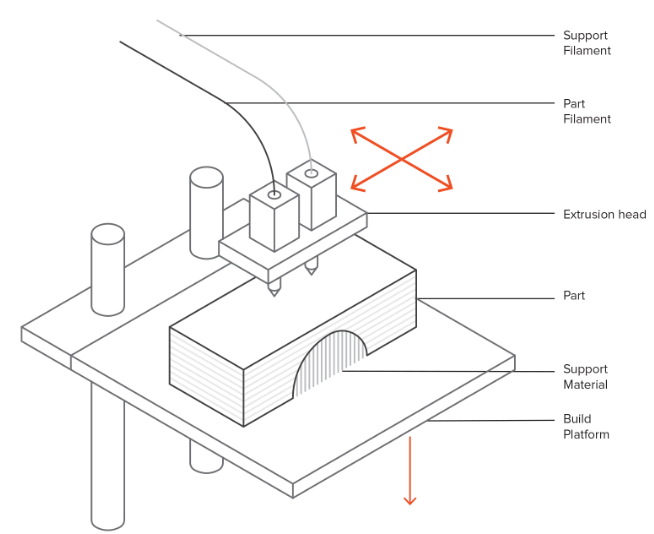
\includegraphics[scale=0.6]{images/fdmesquema.png}
\caption{Esquema de funcionamiento de impresión 3D FDM \citep{bournias2017}.}
\end{figure}
\pagebreak

Dentro de las características principales de este proceso de fabricación se encuentran \citep{bournias2017}:

\begin{description}
\item \textbf{Parámetros de impresión:} la mayoría de los sistemas FDM permiten el ajuste de parámetros del proceso, dentro de los que se incluyen la temperatura de la boquilla y de la plataforma de construcción, velocidad de construcción, altura de capa y velocidad de ventilador de enfriamiento.
\end{description}
\begin{description}
\item \textbf{Adhesión de capa:} Cuando el termoplástico fundido es extruído a través de la boquilla, ejerce una presión sobre la capa previa. La alta temperatura y la presión re-funde la superficie y posibilita la unión con la capa previa. Esto significa que el proceso FDM es ineherentemente anisotrópico: el esfuerzo en el eje-Z es siempre menor que en el plano X-Y.
\end{description}

\begin{description}
\item \textbf{Estructura de Soporte:} Un termoplástico fundido no puede ser depositado en el aire. Por esta razón, algunas geometrías requieren una estructura de soporte, generalmente con una calidad menor que el resto de la pieza.
\end{description}

\begin{description}
\item \textbf{Relleno y ancho de pared:} Usualmente, las piezas impresas en FDM no son sólidas, con el objetivo de reducir el tiempo de impresión y material. Así, los perímetro exteriores son trazados realizando varias pasadas denominadas ancho de pared, mientras que el interior es fabricado con una estructura de baja densidad, llamada relleno.
\end{description}

Por otro lado, los materiales mayoritariamente utilizados por esta tecnología y sus características son: 

\begin{table}[H]
\centering
\begin{tabular}{|c|c|}
\hline
Material & Características \\
\hline
ABS & \parbox{25em}{Alto resistencia, alta resistencia a la temperatura, susceptibilidad a la separación de capas}\\
\hline
PLA & \parbox{25em}{Excelente calidad visual, fácil de imprimir, baja resistencia al impacto}\\
\hline
Nylon (PA) & \parbox{25em}{Alta resistencia, Excelente resistencia química, baja resistencia a la humedad}\\
\hline
PETG & \parbox{25em}{Seguro para alimentos, buena resistencia, fácil de imprimir}\\
\hline
TPU & \parbox{25em}{Muy Flexible, difícil de imprimir}\\
\hline
PEI & \parbox{25em}{Excelente resistencia al peso, ignífugo, Excelente resistencia química, alto costo}\\
\hline
\end{tabular}
\caption{Principales materiales utilizados en impresión 3D FDM \citep{bournias2017}.}
\end{table}

\subsection{Tipologías de impresión 3D FDM}

Si bien el principio de funcionamiento para las impresoras 3D FDM es el mismo, existen diferentes tipologías o modelos de clasificación de éstas. En este caso, se presenta una clasificación según el sistema de coordenadas que utiliza para construir las piezas, donde se distinguen cuatro tipos \citep{b3dsourced2020}:

\begin{description}
\item \textbf{Cartesiana:} Estas impresoras siguen el patrón de coordenadas X, Y y Z para posicionar el cabezal de impresión en el lugar correcto. Existen dos posibilidades de movimiento tanto del cabezal como de la plataforma de construcción: (a) Cabezal móvil en el plano X-Z y plataforma en el eje-Y; (b) Cabezal móvil en el plano X-Y y plataforma en el eje-Z.

\begin{figure}[H]
\centering
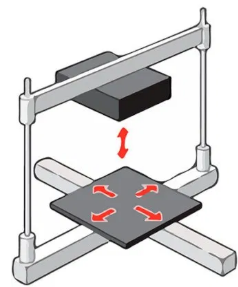
\includegraphics[scale=0.6]{images/cartesiana.png}
\caption{Esquema de impresora 3D cartesiana \citep{b3dsourced2020}.}
\end{figure}

\item \textbf{Delta:} Las impresoras tipo delta incluyen una plataforma de construcción circular y un cabezal unido a tres puntos triangulares fijos. Cada uno de esos tres puntos pueden mover hacia arriba y abajo el cabezal dentro del cilindro de impresión.

\begin{figure}[H]
\centering
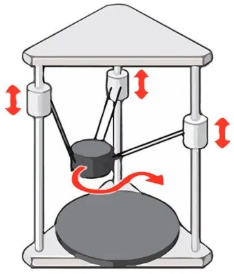
\includegraphics[scale=0.6]{images/delta.png}
\caption{Esquema de impresora 3D Delta \citep{b3dsourced2020}.}
\end{figure}

\item \textbf{Polar:} Esta impresora utiliza un sistema de coordenadas polares, donde cada punto de impresión está determinado por su posición comparada con un punto central en el medio de la plataforma de fabricación.

\begin{figure}[H]
\centering
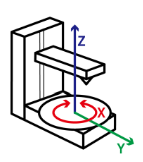
\includegraphics[scale=0.8]{images/polar.png}
\caption{Esquema de impresora 3D polar \citep{takamori2018}}
\end{figure}

\item \textbf{SCARA}: una impresora SCARA (acrónimo de las siglas en inglés Selective Compilant Assembly Robot Arm) maniobra en los ejes X, Y, y Z dentro de un límite de 180 grados. El cabezal de esta máquina se sitúa en un extremo del brazo robot, el cual consta de dos articulaciones giratorias con ejes verticales.

\begin{figure}[H]
\centering
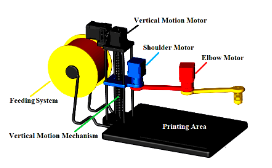
\includegraphics[scale=0.8]{images/scara.png}
\caption{Esquema de impresora 3D scara \citep{saygin2016}}
\end{figure}



\end{description}

\pagebreak
\section{Mantenimiento}

Según la norma ISO-14224:2016, el mantenimiento se define como una combinación de todas las técnicas y acciones de gestión destinadas a mantener un item o restablecerlo, a un estado en el cual su desempeño es requerido \citep{iso2016}. De una manera más amplia, el concepto de mantenimiento puede establecerse según distintas formas dado el enfoque que se dé en cada caso. Un punto de partida, es mantener el correcto estado funcional de los equipos e instalaciones, sin embargo, las consecuencias que el desarrollo de este principio elemental puede tener sobrepasan ampliamente el objetivo inicial \citep{gomez1998}. En este sentido, y buscando una definición global, se puede decir que el mantenimiento corresponde al conjunto de técnicas destinado a conservar equipos e instalaciones en servicio durante el mayor tiempo posible (buscando la más alta disponibilidad) y con el máximo rendimiento \citep{garcia2010}.
Teniendo en cuenta factores como el tipo de industria y su tamaño, la política de la empresa, las características de la producción, el campo de acción de las actividades de un departamento de ingeniería de mantenimiento puede incluir las siguientes responsabilidades\citep{gomez1998}: \\

\begin{itemize}
\item Mantener los equipos e instalaciones en condiciones operativas, eficaces y seguras.
\item Efectuar un control del estado de los equipos, así como de su disponibilidad.
\item Realizar los estudios necesarios para reducir el número de averías imprevistas.
\item En función de los datos históricos disponibles, efectuar una previsión de los repuestos de almacén necesarios.
\item Intervenir en los proyectos de modificación del diseño de equipos e instalaciones.
\item Llevar a cabo aquellas tareas que implican la modificación o reparación de los equipos e instalaciones.
\item Instalación de nuevo equipo.
\item Asesorar a los mandos de producción.
\item Velar por el correcto suministro y distribución de energía.
\item Tareas de vigilancia.
\end{itemize}

\subsection{Historia y evolución del mantenimiento}

Si bien no existe precisión histórica o documentación para establecer los orígenes del mantenimiento ya sea, por ejemplo, en la diferencia entre la evolución de las distintas industrias, la literatura sí genera distintos consensos en lo que respecta a ciertos hitos que pueden dar luces a este contexto histórico. En este sentido, las principales referencias que existen en diversas fuentes bibliográficas sobre los tipos de mantenimiento llevados a cabo han concluido, de común acuerdo entre muchos autores, en establecer durante el siglo XX tres grandes etapas que, aunque no tienen una una frontera clara desde el punto de vista temporal, si pueden dar una clara idea de cómo ha sido la evolución de las técnicas y organizaciones que se han implementado durante dicho siglo. Se ha convenido entonces, que la evolución del mantenimiento ha tenido tres etapas, a las cuales se les denomina \textit{primera, segunda} y \textit{tercera generación} \citep{gonzalez2005}.
Así, el comienzo del siglo XX marca efectivamente el inicio de las actividades de mantenimiento reparativo y la creación de los primeros talleres que originan la \textit{Primera Generación} del mantenimiento, que se extiende hasta mediados del siglo y tiene como características relevantes \citep{garcia2012}:

\begin{itemize}
\item Equipos robustos, sobredimensionados y simples.
\item Volúmenes de producción bajos.
\item Las actividades demandaban poca destreza.
\item No existía la alta mecanización industrial
\item Poca importancia a los tiempos de parada de los equipos.
\item La prevención de fallas en los equipos no era prioridad.
\item El mantenimiento era mantenimiento reactivo o de reparación.
\item No había necesidad de un mantenimiento sistemático.
\end{itemize}  

Esta etapa, la más larga desde la revolución industrial hasta después de la Segunda Guerra Mundial, se caracteriza esencialmente por la corrección de averías, reengrases, lubricaciones y limpiezas \citep{gonzalez2005}.

En tiempos posteriores a la guerra se vio la necesidad de implantar técnicas con el fin de prevenir las fallas de los equipos en combate y disminuir los costos de reparación, por lo que vino a tomar importancia relevante la disponibilidad y duración de vida útil de la maquinaria \citep{garcia2012}. El descubrimiento de relación entre edad de equipos y probabilidad de fallos, junto a la enorme competencia industrial, además de la incorporación de los fabricantes orientales al mundo competitivo occidental, es uno de los desencadenantes de una continua búsqueda de mejores resultados. En esta etapa denominada \textit{segunda generación}, se ponen en marcha sistemas de mantenimiento preventivo basados en revisiones cíclicas de equipos, instalaciones y medios en general \citep{gonzalez2005}. Dentro de las características principales de este periodo se señalan \citep{garcia2012}:

\begin{itemize}
\item Importancia de la productividad
\item Incremento de la mecanización en las industrias
\item Aumento de la complejidad de los equipos
\item Mayor interés a los tiempos de parada de los equipos
\item Inicio del mantenimiento preventivo
\item Altos niveles de inventario de repuestos
\item Crecimiento de los costos de mantenimiento
\item Sistemas de planificación y control de mantenimiento
\item Aumento de la vida útil de los equipos y sistemas
\item Inicio de la sistematización del Mantenimiento
\end{itemize}

La optimización de este mantenimiento de segunda generación, basado por tanto en mantenimientos preventivos rutinarios y mantenimiento correctivo, se fundamenta en avanzados sistemas de planificación de actividades y de control de trabajos realizados; entendiendo por control tanto el lanzamiento de órdenes de trabajo como la retroalientacnión y verificación de los datos habidos en esas órdenes de trabajo \citep{gonzalez2005}.

Se debe decir que, durante el periodo posterior a 1980, se han visto los peores accidentes en la historia de la industria mundial. Las filtraciones de baterías en Bhopal, India, o  la amenaza a la supervivencia de la humanidad causada por el accidente nuclear de Chernobyl, solo han hecho que la industria realce la importancia del mantenimiento \citep{shenoy2005}. Este punto de inflexión, sumado a las preocupaciones que ya existían ciertos postulados en relación a la máxima calidad, seguridad y protección del medio ambiente, dio origen a la tercera generación del mantenimiento, que se extendió hasta el final del siglo \citep{garcia2012}. Cabe destacar que en el mantenimiento de tercera generación, la observancia de normativa adquiere una importancia primordial. Son muchas las administraciones estatales, autonómicas y locales que abordan reglamentaciones específicas del mantenimiento; así pues, aparecen reglamentos para aparatos a presión, equipos de manutención y transporte, ascensores y escaleras mecánicas, etc. Este aspecto toma también relevancia y define lo que se ha convenido en llamar, dentro de los mantenimientos preventivos, mantenimientos legales o reglamentarios \citep{gonzalez2005}. Dentro de los parámetros más importantes involucrados en esta generación del mantenimiento se encuentran \citep{louis2012}:

\begin{itemize}
\item Disponibilidad y confiabilidad de los equipos
\item Mayor seguridad
\item Eliminar el daño al Medio Ambiente
\item Mejor calidad de producción
\item Mayor vida útil de los equipos
\item Efectividad en los costos.
\end{itemize}

Asimismo, las técnicas asociadas a este periodo de tiempo son \citep{louis2012}:\\

\begin{itemize}
\item Monitoreo de la condición
\item Diseños para la mantenibilidad y confiabilidad
\item Computadores pequeños y rápidos
\item Analisis de modos y efectos de falla
\end{itemize}     

La añadidura tanto de nuevos desafíos y de las técnicas que hacen frente a éstos, revelan que  las tres generaciones anteriormente mencionadas plantean la necesidad de coexistir en un mantenimiento equilibrado y acondicionado a la realidad de la industria. De esto se obtiene que la primera generación define las acciones del mantenimiento reactivo, la segunda plantea la estrategia de revisiones cíclicas, y la tercera generación la estrategia basada en la condición \citep{hide2013}.
Así, la cuarta generación del mantenimiento es también el entendimiento que tanto el mantenimiento preventivo, como el correctivo o el predictivo juega un rol en la optimización de la disponibilidad, confiabilidad y el costo de los activos industriales. En este caso, son importantes las técnicas avanzadas como la recolección de data a través de sensores o la analítica de softwares \citep{houle2016}.
En tanto a los procesos, la tecnología de la información, el uso y la disponibilidad del internet, la obtención de información en cualquier parte del mundo y el entendimiento de estos son reconocidos como los conductores hacia los nuevos entendimientos del mantenimiento.


\subsection{Mantenimiento correctivo}

El estándar ISO-14224-2016 define el mantenimiento correctivo como el mantenimiento realizado después de la detección de fallas, con objeto de efectuar su restauración \citep{iso2016}. Este tipo de mantenimiento, también llamado mantenimiento a rotura, sólo se interviene en los equipos cuando el fallo ya se ha producido. Se trata, por tanto, de una actitud pasiva, frente a la evolución del estado de los equipos, a la espera de la avería o fallo \citep{gomez1998}. De la misma forma, el mantenimiento correctivo es el conjunto de tareas destinadas a corregir los defectos que se van presentando en los distintos equipos y que son comunicados al departamento de mantenimiento por los usuarios de los mismos \citep{garcia2010}.
Adoptar esta forma de mantenimiento supone asumir algunos inconvenientes respecto a las máquinas y equipos afectados, entre los que pueden citarse \citep{gomez1998}:\\

\begin{itemize}
\item Las averías se producen generalmente de forma imprevista, lo que puede ocasionar trastornos en la producción, que pueden ir desde ligeras pérdidas de tiempo, por reposición de equipo o cambio de tarea, hasta la parada de la producción, en tanto no se repare o sustituya el equipo averiado.
\item Las averías, al ser imprevistas, suelen ser graves para el equipo, con o que su reparación puede ser costosa.
\item Las averías son siempre -en mayor o menor medida- inoportunas, por lo que la reparación de los equipos averiados puede llevar más tiempo del previsto, ya sea por ausencia del personal necesario para su reparación, o ya sea por la falta de los repuestos necesarios.
\item Por tratarse de averías inesperadas, el fallo podría venir acompañado de algún siniestro, lo que obviamente puede tener consecuencias muy negativas para la seguridad del personal y las instalaciones.
\end{itemize}

De aquellas empresas donde el 100\% del mantenimiento es correctivo, se podría considerar que, en promedio, en más del 70\% del tiempo total dedicado a mantener sus activos se utiliza para la solución de fallas no programadas; por tanto, gestionar con eficacia el mantenimiento correctivo significa \citep{garcia2010}:

\begin{itemize}
\item Realizar intervenciones con rapidez, que permitan la puesta en marcha del equipo en el menor tiempo posible (MTTR o tiempo medio para reparar bajo).
\item Realizar intervenciones fiables, y adoptar medidas para que no se vuelvan a producir estas en un periodo de tiempo suficientemente largo (MTBF o tiempo medio entre fallos grande).
\item Consumir la menor cantidad posible de recursos (tanto mano de obra como materiales).
\end{itemize}

\subsection{Mantenimiento preventivo}

El estándar ISO-14224-2016 presenta el mantenimiento preventivo planificado como el mantenimiento realizado de acuerdo a una planificación específica \citep{iso2016}. En este sentido, este tipo de mantenimiento pretende evitar la reparación mediante una rutina de inspecciones periódicas y la renovación de los elementos deteriorados. En estas inspecciones, se procede al desmontaje total o parcial de la máquina con el fin de revisar el estado de sus elementos, reemplazando aquellos que se estime oportuno a la vista del examen realizado. Otros elementos son sustituidos sistemáticamente en cada inspección, tomando como referencia el número de operaciones realizadas o un determinado periodo de tiempo de funcionamiento \citep{gomez1998}. Dicho esto, existen autores que plantean modelos donde estos tipos de mantenimiento estén involucrados y compartan otras actividades, con el fin de hacer más rentable las acciones determinadas. Uno de estos modelos es el mantenimiento preventivo sistemático, el cual incluye un conjunto de tareas que se realizarán sin importar la condición del equipo. Es importante señalar que un equipo sujeto a un modelo de mantenimiento sistemático no tiene por qué tener todas sus tareas con su periodicidad fija. El mantenimiento preventivo sistemático contempla \citep{garcia2010}:

\begin{itemize}
\item Inspecciones visuales.
\item Lubricación.
\item Mantenimiento preventivo planificado.
\item Mantenimiento condicional.
\item Reparación de averías.
\end{itemize}

Dentro de las principales ventajas de este tipo de mantenimiento están \citep{jimenez2015}:

\begin{itemize}
\item Conocimiento del estado de funcionamiento de las instalaciones.
\item Mejora de las condiciones de seguridad laborales.
\item Aumento de la vida útil de las instalaciones.
\item Mayor rendimiento de trabajadores y máquinas debido a la eliminación de tiempos muertos.
\item Disminución en los costes de reparación de averías.
\end{itemize}

Según Jimenez (2015), los principales inconvenientes son:

\begin{itemize}
\item Los elementos son cambiados antes de que estos lleguen a su vida útil completa.
\item Si no se realiza una buena programación de operaciones y con una frecuencia óptima, con este tipo de mantenimiento se pueden aumentar los costes, así como la disminución del rendimiento de las máquinas o instalaciones.
\end{itemize}

Para que un mantenimiento preventivo sea efectivo, deberá seguir los siguientes pasos \citep{jimenez2015}:

\begin{enumerate}
\item Saber los objetivos del trabajo.
\item Conocer el programa de mantenimiento preventivo y predictivo.
\item Seleccionar los equipos para realizar el mantenimiento.
\item Recoger información de los equipos susceptibles de mantenimiento.
\item Estudio de la información obtenida.
\item Estudio de los métodos de trabajo así de cómo las desviaciones de las operaciones de mantenimiento.
\item Análisis y conclusiones de las operaciones de mantenimiento realizadas.
\item Presentación de las propuestas de mejora.
\item Estudio de propuestas de mejora y posibilidad de nueva frecuencia del mantenimiento preventivo.
\item Estudio y análisis de los resultados.
\item Actualización del programa de mantenimiento.
\end{enumerate}



\subsection{Mantenimiento centrado en la condición}


Respecto al mantenimiento centrado en la condición de equipos y las normas que definen su marco de trabajo, se encuentra la norma ISO 13372:2012 la cual se refiere al vocabulario relacionado al monitoreo de la condición y su diagnóstico, y el estándar ISO 17359-2018 que presenta las guías generales para el proceso anteriormente mencionado.
Las perspectivas del proceso de monitoreo de la condición se presentan a través de un diagrama que detalla los pasos necesarios para dirigir las actividades de monitoreo para identificar y evitar modos de falla \citep{iso2018}. 
Al mismo tiempo, el estándar propone una diversidad de análisis a tener en cuenta para el monitoreo de la condición, entre los que se encuentran \citep{iso2018}:

\begin{description}
\item \textbf{Análisis costo beneficio:} un análisis inicial de factibilidad y costo beneficio ayuda a establecer indicadores de desempeño precisos y referencias para medir la efectividad de cualquier programa de monitoreo de la condición. Los ítem a considerar incluyen:
\begin{itemize}
\item Ciclo de costo de vida.
\item Costo de la producción perdida.
\item Daño consecuente.
\item Garantías y seguros.
\end{itemize}

\item \textbf{Identificación del equipo:} Se establece un esquema genérico de una máquina y sus distintos componentes y procesos para considerar la gestión del monitoreo de la condición. Entre ellos se encuentran: estructura; tuberías; lubricación; sistemas de control; configuración y rangos; entradas y salidas; personal; medio ambiente; sistemas de protección; data; técnicas de monitoreo de la condición; posición y accesibilidad; máquinas adyacentes.

\item \textbf{Identificación de la función del equipo:} Se busca identificar la siguiente información: (a) qué debe realizar el sistema, máquina o equipamiento; (b) cuáles son las condiciones de operación de la máquina o sistema, o el rango de condiciones de operación.

\item \textbf{Equipos críticos:} se recomienda una evaluación crítica de todas las máquinas, para crear una lista de prioridades y ser incluidas (o no) en el programa de monitoreo de la condición. Puede ser un sistema simple de calificación basado en los siguientes factores:

\begin{itemize}
\item Costo de máquina fuera de servicio o pérdida de costos de producción.
\item Rango de falla y tiempo medio para reparar.
\item Redundancia.
\item daño secundario.
\item Costo de reemplazo de la máquina.
\item Costo del mantenimiento.
\item Costo del ciclo de vida.
\item Costo del sistema de monitoreo.
\item Seguridad e impacto medioambiental.
\end{itemize}

\item \textbf{Técnicas de medición:} Para la medición particular de los parámetros considerados, pueden ser apropiadas una o más mediciones. Los parámetros de éstas pueden ser simples mediciones de valores generales, o valores promediados en el tiempo. Para ciertos parámetros como voltaje, corriente o vibraciones, puede que este tipo de mediciones no sean suficientes para mostrar la ocurrencia de una falla.

\item \textbf{Exactitud de los parámetros de monitoreo:} En la mayoría de los casos, la exactitud de los parámetros requeridos para ser usado en el monitoreo y diagnostico de la condición de la máquina no es necesariamente tan absoluto como la precisión que se podría requerir para otras mediciones, como pruebas de rendimiento.

\item \textbf{Condiciones de operación durante el monitoreo:} Si es posible, el monitoreo debe ser llevado a cabo cuando la máquina ya ha alcanzado una configuración predeterminada de las operaciones de condición. Mediciones de diferentes parámetros deben ser tomados siempre que sea posible y al mismo tiempo bajo las mismas condiciones de operación.

\item \textbf{Intervalos de monitoreo:} Se debe considerar el intervalo entre mediciones, y si se requiere un muestreo continuo o periódico. El intervalo primario del monitoreo depende del tipo de falta, su rango de progresión y el rango de cambio de los parámetros relevantes. El tiempo transcurrido entre la detección de la falta y la falla actual es conocido como tiempo de espera para fallar (LTTF).

\item \textbf{Registro de parámetros de monitoreo:} el regitro de parámetros de monitoreo debe incluir, como mínimo, la siguiente información:
\begin{itemize}
\item Data esencial que describe la máquina.
\item Data esencial que describe la condición de operación.
\item Posición de medición.
\item Unidades y procesamiento de medición.
\item Información sobre fecha y hora.
\end{itemize}

\item \textbf{Criterio de alerta inicial:} el criterio de alerta inicial debe ser configurado  como el más temprano indicador posible de la ocurrencia de una falta. Las alarmas deben ser valores unitarios o de niveles múltiples, donde ambos incrementan y/o decrecen. 

\item \textbf{Data Base o referencia:} Esta data es medida u observada cuando la operación del equipo se conoce como aceptable o estable. 

\item \textbf{Diagnóstico y pronóstico:} el proceso de diagnóstico es generalmente provocado por una detección anormal. Esta detección es llevada a cabo realizando una comparación entre los descriptores presentes de la máquina, o comparando con una máquina similar.

\item \textbf{Determinar acciones de mantenimiento:} la acción más simple que puede ser tomada en ciertas circunstancias es decidir el llevar a cabo una acción no inmediata,  y continuar el monitoreo a intervalos normales. en caso de ocurrencia de una falta, las decisiones incluyen lo siguiente:
\begin{itemize}
\item Sin acción, continuar con el monitoreo de rutina.
\item Reducir el intervalo a la siguiente medición requerida.
\item cambiar la carga o velocidad de la máquina.
\item Apagar la máquina.
\item Inspeccionar la máquina o adelantar mantenimiento de rutina planificado.
\item Llevar a cabo mantenimiento correctivo.

\end{itemize}
\end{description}




\subsection{Mantenimiento centrado en la confiabilidad}



El Mantenimiento Centrado en Confiabilidad (RCM) corresponde a un procedimiento basado en el sentido común con un diagrama de decisión para la creación de estrategias de mantenimiento para proteger las funciones de los activos. RCM se define como un proceso para determinar qué debe hacerse para mantener los activos físicos funcionando de acuerdo a lo que sus operadores quieren que éstos hagan en su contexto operacional actual \citep{sifonte2017}.
El estándar internacional ISO 14224-2016 reúne los criterios para la colección e intercambio de data de mantenimiento y confiabilidad para los equipos. Por otra parte, los criterios que todo proceso debe cumplir para ser llamado RCM son establecidos en la norma SAE JA1011, publicada en 1999. respecto a la primera, se plantean las siguientes definiciones \citep{iso2016}:\\

\begin{description}
\item \textbf{Ciclo medio de Falla (MCTF):} número de ciclos esperado antes de que el item falle.
\item \textbf{Número medio de ciclos:} número esperado de ciclos por unidad de tiempo.
\item \textbf{Tiempo medio de reparación activa (MART):} tiempo esperado para reparación activa.
\item \textbf{Tiempo medio transcurrido entre fallas (METBF):} tiempo medio transcurrido esperado entre fallas sucesivas de un ítem reparable.
\item \textbf{Tiempo medio de reparación general:} tiempo esperado para lograr las siguientes acciones: tiempo gastado antes de comenzar la reparación y; tiempo anterior en que el ítem esté disponible para volver a operación
\item \textbf{Tiempo medio para falla (MTTF):}: tiempo esperado antes de que un ítem falle.
\item \textbf{Tiempo medio para reparar (MTTR):} tiempo esperado para lograr la reparación un ítem fallado.
\end{description}

Por otra parte, la norma SAE JA1011 establece siete pasos descritos a continuación:\\

\begin{itemize}
\item Delimitar el contexto operativo, las funciones y los estándares de desempeño asociados al activo (contexto operacional y funciones.
\item Determinar cómo un activo puede fallar en el cumplimiento de sus funciones (fallas funcionales).
\item Definir las causas de cada falla funcional (modos de falla).
\item Describir qué sucede cuando ocurre cada falla (efectos de falla).
\item Clasificar los efectos de las fallas (consecuencias de la falla).
\item Determinar qué se debe realizar para predecir o prevenir cada falla (tareas e intervalos de tareas).
\item Decidir si otras estrategias de gestión de fallas pueden ser más efectivas (cambios de una sola vez). 
\end{itemize}

Para el cumplimiento de los pasos anteriores, la norma determina una serie de definiciones dentro de las cuales se encuentran \citep{saeja1011}:\\

\begin{itemize}
\item[$ $] \textbf{Función:} lo que un usuario espera que realice un activo físico o sistema.
\item[$ $] \textbf{Falla Evidente:} Modo de falla cuyos efectos se vuelven evidentes para los operarios bajo circunstancias normales si el modo de falla ocurre por si mismo o aislado.
\item[$ $] \textbf{Función Evidente:} Función cuya falla sobre si mismo se vuelven aparentes para los operarios bajo circunstancias normales.
\item[$ $] \textbf{Fallas Funcionales:} Estado en el cual un activo físico o sistema no es capaz de ejercer una función específica a un nivel de desempeño deseado.
\item[$ $] \textbf{Modos de falla:} Evento único, que provoca una falla funcional.
\item[$ $] \textbf{Efectos de falla:} Lo que ocurre cuando se produce un modo de falla.
\item[$ $] \textbf{Consecuencias de la falla:} las formas en las cuales importan los modos de falla o múltiples fallas. 
\item[$ $] \textbf{Falla oculta:} Modo de falla cuyos efectos no son evidentes para los operarios bajo circunstancias normales si el modo de falla ocurre por si mismo.
\item[$ $] \textbf{Falla múltiple:} Evento que ocurre si la función protegida falla mientras un sistema se encuentra en estado de falla.
\item[$ $] \textbf{Probabilidad condicional de una falla:} La probabilidad de que una falla ocurra en un periodo específico, siempre que el item en cuestión haya sobrevivido desde el principio de ese periodo.

\end{itemize}

Respecto al establecimiento de los modos de falla, la norma en cuestión recomienda cierta profundidad en el nivel de causalidad de los modos de falla. Cuando éstos se enumeren, se debe considerar \citep{saeja1011}:\\

\begin{itemize}
\item Identificar todos los modos de falla razonablemente propensos a causar cada falla funcional.
\item El método utilizado para decidir qué constituye un modo de falla.
\item El nivel de causalidad para los modos de falla debe ser suficientemente exhaustivo para puedan asignar políticas de gestión de fallos.
\item Los modos de falla enumerados en el análisis deben considerar los eventos que han ocurrido antes, los modos de falla que se previenen en las tareas programadas existentes y otros eventos que es probable que se produzcan en el contexto operacional real, pero que nunca ha ocurrido.
\item Los errores humanos y de diseño que causan un evento de falla deben incluirse en la lista de modos de falla, al menos que estén siendo abordados por otros métodos de análisis.

\end{itemize}

En torno a los efectos de falla, se recomienda describir lo que ocurre cuando se produce el modo de falla, teniendo en cuenta lo siguiente \citep{saeja1011}:\\

\begin{itemize}
\item ¿Hay alguna evidencia de que ha ocurrido una falla?
\item ¿Cuál es el impacto potencial que tiene la falla en la seguridad del personal?
\item ¿Cuál es el impacto potencial que tiene la falla en el medio ambiente?
\item ¿Cómo se ve afectada la producción o las operaciones?
\item ¿Hay algún daño físico causado por la falla?
\item ¿Hay algo que deba hacerse para restaurar la función del sistema después de la falla? 
\end{itemize}

Los efectos de fallas se deben clasificar en categorías basadas en la evidencia que se tiene de éstas, impactos en la seguridad, medio ambiente, capacidad operacional y costos. Se debe elegir una categoría para cada efecto de modo de falla, haciendo énfasis en la que sea más grave \citep{sifonte2017}.

La norma SAE JA1011 reconoce cinco posibles estrategias de mantenimiento que deben ser aplicadas para mitigar las consecuencias de las fallas\citep{sifonte2017}:\\

\begin{itemize}
\item[$ $] \textbf{Mantenimiento Basado en la Condición:} Estas tareas están destinadas a detectar fallas potenciales. Tal detección debe ocurrir con suficiente antelación para que la acción correctiva se pueda tomar antes de un paro operacional. Una tarea de monitoreo de condición es aplicada a intervalos fijos para predecir la tendencia de un paro operacional antes de que ocurra una falla funcional.
\item[$ $] \textbf{Tareas de reparaciones programadas:} Las tareas de reparación basadas en el tiempo deben ser realizadas en función de la vida útil del activo. Es decir, el momento en que la tasa de falla del equipo deja de ser constante. En teoría, al final de la vida útil, la tasa de falla del activo aumenta más allá de lo que podemos tolerar. Además de la vida útil, el costo de la reparación preventiva también necesita ser evaluado. Esto es, una comparación del costo del trabajo de reparación contra el de las consecuencias de la falla funcional debe confirmar la viabilidad económica de la tarea.
\item[$ $] \textbf{Tareas de reemplazo programado:} Las tareas programadas de descarte y reemplazo se consideran cuando se demuestra que es más rentable reemplazar que reparar el activo. Se recomienda aplicar dicha sustitución al final de la llamada vida “útil” del mismo.
\item[$ $] \textbf{Tareas de búsqueda de fallas:} Estas tareas están destinadas a detectar fallas ocultas asociadas, la mayoría de las veces, con dispositivos de protección o componentes redundantes. Debemos asegurarnos de que es físicamente posible realizar la tarea de búsqueda recomendada y que la frecuencia sugerida es aceptable para el propietario del activo. En el libro se hablará más sobre la frecuencia de la tarea.
\item[$ $] \textbf{Tareas de búsqueda de rediseño:} Los cambios en la configuración física de los activos, los procedimientos de operación o mantenimiento, el adiestramiento del operador / mantenedor y la alteración del contexto operacional son todas las formas posibles de cambios de una sola vez o rediseño potencialmente necesario para la mitigación de fallas.

\end{itemize}


\subsection{Confiabilidad}

La confiabilidad puede ser definida como la confianza que se tiene de que un componente, equipo o sistema desempeñe su función básica, durante un periodo de tiempo preestablecido, bajo condiciones estándares de operación; otra definición es la probabilidad de que un ítem pueda desempeñar su función requerida durante un intervalo establecido y bajo condiciones de uso definidas \citep{dairo2016}. Existen diversos modelos matemáticos que pueden describir el comportamiento de una variable a través del tiempo, los cuales se enuncian a continuación:

\subsubsection{Función densidad de probabilidad}

La función densidad de probabilidad puede describir la distribución de la probabilidad de una variable aleatoria continua $X$. Así, una función de densidad de probabilidad es una función tal que:


 $$f(x)\geqslant 0$$
 $$\int_{-\infty}^{\infty}f(x)dx=1$$
 \begin{equation*}
 P(a\geqslant X \geqslant b)=\int_{a}^{b}f(x)dx= \text{ área bajo } f(x) \text{ de } a \text{ a } b, \text{ para cualquier } a \text{ y } b.
 \end{equation*}



Esta función proporciona una descripción simple de las probabilidades asociadas a una variable aleatoria.

\subsubsection{Media y varianza de una variable continua}

Si se tiene que $X$ es una variable aleatoria continua con función de densidad de probabilidad $f(x)$, se define la Media de $X$ como:

\begin{equation}
\mu=E(X)=\int_{-\infty}^{\infty}xf(x)dx
\end{equation}

Asimismo, la Varianza de $X$:

\begin{equation}
\sigma^2=V(X)=\int_{-\infty}^{\infty}(x-\mu)^{2}f(x)dx=\int_{-\infty}^{\infty}x^{2}f(x)dx-\mu^2
\end{equation}

La Desviación Estandar:

\begin{equation}
\sigma=\sqrt{V(X)}
\end{equation}

\subsubsection{Distribución normal}

Variables aleatorias con medias y varianzas diferentes pueden modelares por medio de funciones de densidad de probabilidad normal, con la elección adecuada del centro y anchura de la curva. La función de densidad de probabilidad normal se define como:

\begin{equation}
f(x)=\frac{1}{\sqrt{2\pi\sigma}}e^{\frac{-(x-\mu)^2}{2\sigma^2}}  ,  -\infty<x<\infty
\end{equation}

tiene una distribución normal con parámetros $\mu$, donde $-\infty<\mu<\infty$, y $\sigma>0$.\\

Además,
\begin{equation}
E(X)=\mu , V(x)=\sigma^2
\end{equation}

\subsubsection{Distribución exponencial}

La distribución exponencial debe su nombre a la función exponencial de la función de densidad de probabilidad. Así, la variable aleatoria $X$ (que es igual a la distancia entre conteos sucesivos de un proceso de Poisson con media $\lambda>0$ tiene una distribución exponencial con parámetro $\lambda$:

\begin{equation}
f(x)=\lambda e^{-\lambda x}, 0<x<\infty
\end{equation}

Si la variable tiene una distribución exponencial con parámetro $\lambda$:

\begin{equation}
E(x)=\frac{1}{\lambda}, V(X)=\frac{1}{\lambda^2}
\end{equation}

\subsubsection{Distribución de Weibull}

La distribución de Weibull se utiliza con frecuencia para modelar el tiempo hasta que ocurre una falla en algún sistema. La función de densidad de problabilidad para la distribución está definida como:

\begin{equation}
f(t)=\frac{\beta\cdot t^{\beta-1}}{\theta^\beta}\cdot exp\left[-\left(\frac{t}{\theta}\right)^\beta\right] \quad t\geq 0,\text{ }\theta>0,\text{ }b>0 
\end{equation}

Donde $\beta$ y $\theta$ son los parámetros forma de y escala de la distribución, respectivamente; mientras que $t$ corresponde a la variable aleatoria que en el caso de la confiabilidad responde al tiempo entre fallas.

La función confiabilidad de Weibull se determina como:

\begin{equation}
R(t)=\int_{s}^{\infty}f(s)ds= exp\left[-\left(\frac{t}{\theta}\right)^\beta\right]
\end{equation}

Por otro lado, la función de distribución acumulativa está dad por la ecuación

\begin{equation}
R(t)=1-F(t)\quad R(t)=1-exp-\left[\left( \frac{t}{\theta}\right)^\beta\right]
\end{equation}

Utilizando el método de mínimos cuadrados para obtener los parámetros de forma y escala, aplicado a la función de distribución acumulativa:

\begin{equation}
F(t)=1-exp\left[-\left(\frac{t}{\theta}\right)^\beta\right]
\end{equation}

\begin{equation}
\rightarrow \frac{1}{exp \left[\left(\frac{t}{\theta}\right)^\beta\right]}=1-F(t)
\end{equation}

\begin{equation}
\rightarrow \frac{1}{1-F(t)}=exp\left[\left(\frac{t}{\theta}\right)^\beta\right]
\end{equation}

Aplicando logaritmo natural:

\begin{equation}
\rightarrow ln\left(\frac{1}{1-F(t)}\right)=ln\left[exp\left[\left(\frac{t}{\theta}\right)^\beta \right]\right]
\end{equation}

\begin{equation}
\rightarrow ln\left( \frac{1}{1-F(t)} \right)=\left( \frac{t}{\theta}\right)^\beta 
\end{equation}

Calculando nuevamente el logaritmo natural para la expresión anterior:

\begin{equation}
\rightarrow ln\left[ln\left[\frac{1}{1-F(t)}\right]\right]=\beta\cdot ln\left(\frac{t}{\theta}\right)
\end{equation}

\begin{equation}
\rightarrow ln\left[ln\left[\frac{1}{1-F(t)}\right]\right]=\beta ln(t)-\beta ln(\theta)
\end{equation}

Luego, se obtiene una ecuación lineal de la forma $y=ax-b$. Se debe notar que $\beta$ corresponde a la pendiente de la ecuación. Como se éste se define como el factor de forma, surgen las siguientes consideraciones:

\begin{description}
\item Cuando $\beta<1$ existen desgastes en que la tasa de fallos disminuye en función del tiempo, luego de un incremento repentino. Si $\beta\rightarrow0$, se asocia a ciclos de desgaste bajo; por otra parte, cuando $\beta\rightarrow1$, existen ciclos de desgaste altos. Asimismo, un valor de $\beta$ menor a uno indica fallos infantiles.
\item Cuando $\beta>1$, se trata de desgaste debido a la disminución constante de la resistencia antes de su puesta en servicio.
\end{description}

\pagebreak

\section{Lean Manufacturing}

Lean Manufacturing como definición, corresponde a una filosofía de trabajo, basada en las personas, que define la forma de mejora y optimización de un sistema de producción focalizándose en identificar y eliminar todo tipo de desperdicios, definidos éstos como aquellos procesos o actividades que usan más recursos de los estrictamente necesarios \citep{hernandez2013}. Desde el punto de vista de los sistemas, el sistema de gestión Lean (SGL) es un sistema de gestión metódico y ordenado, basado en la eliminación del desperdicio, que dota a todos los trabajadores de reglas sociales y de actuaciones eficientes para conducirlos hacia la mejora de su desempeño de forma constante y tenaz \citep{leansis2017}. Lean manufacturing es una tarea incansable e ininterrumpida para crear empresas más efectivas, innovadoras y eficientes. A partir de esta filosofía se han desarrollado una diversidad de aplicaciones, tanto en manufactura como en servicios. Actualmente, dentro de los casos de éxito en los que se desarrolla Lean se pueden considerar \citep{socconini2019}:

\begin{itemize}
\item Lean Manufacturing (manufactura ágil).
\item Lean Government (administraciones públicas ágiles).
\item Lean Office (oficinas ágiles).
\item Lean Design (diseño ágil).
\item Lean Logistics (logística ágil).
\end{itemize}

Una forma de visualizar la filosofía que encierra Lean y las técnicas disponibles es el esquema de \textit{Casa del Sistema de Producción Toyota}. Se explica utilizando una casa puesto que esta constituye un sistema estructural que es fuerte siempre desde sus cimentos hasta sus columnas. Una adaptación actualizada de esta casa es la siguiente \citep{leansis2017}:


\begin{figure}
\centering
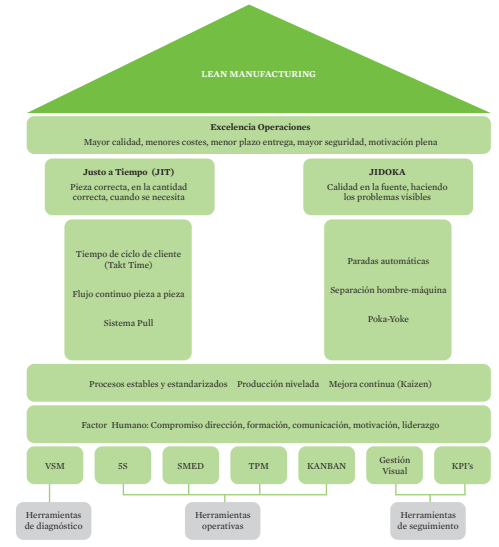
\includegraphics[scale=0.8]{images/casalean.png}
\caption{Esquema actualizado de la Casa Toyota \citep{leansis2017} }
\end{figure}
 

Otra forma de explicar la fundamentación de Lean Manufacturing, es a través de ciertos principios desde el punto de vista del factor humano, la manera de trabajar y pensar \citep{leansis2017}:

\begin{itemize}
\item Trabajar en la planta y comprobar las cosas in situ.
\item Formar líderes de equipos que asuman el sistema y lo enseñen a otros.
\item Interiorizar la cultura de \textit{parar la línea}.
\item Desarrollar personas involucradas que sigan la filosofía de la empresa.
\item Respetar a la red de suministradores y colaboradores ayudándoles y proponiéndoles retos.
\item Identificar y eliminar funciones y procesos que no son necesarios.
\item Promover equipos y personas multidisciplinares.
\item Descentralizar la toma de decisiones.
\item Integrar funciones y sistemas de información.
\item Obtener el compromiso total de la dirección con el modelo Lean.
\end{itemize}

\subsection{Historia Lean Manufacturing}

Los antecedentes de la manufactura de remontan al año 1776, cuando James Watt inventó la máquina a vapor de doble acción, hecho que marcó el inicio de la Revolución Industrial. A este hito, se suman posteriormente los estudios del trabajo de Administración Científica de Frederick Taylor, que institucionalizó el sistema de producción con lotes, y propuso la división en departamentos que centran sus esfuerzos en actividades específicas, que devino posteriormente en un modelo para la industria industrial y la estandarización del trabajo; a esto se suma la contribución de Henry Ford y la creación del automovil modelo T, que dio lugar en 1915 a la creación de su linea de ensamble, revolucionando la manera de trabajar en la manufactura \citep{socconini2019}. La ruptura de estas técnicas se produce en Japón, donde se encuentra el primer germen del pensamiento Lean. En 1902, Sakichi Toyoda, inventó un dispositivo que detenía el telar cuando se rompía el hilo e indicaba con una señal visual al operador que la máquina necesitaba atención. Este sistema permitió separar al hombre de la máquina, dando la oportunidad a un único operario la capacidad de controlar varios dispositivos. en 1929, Toyoda vende los derechos de sus patentes de telares a la empresa Británica Platt Brothers, y encarga a su hijo Kiichiro que invierta en la industria automotriz, naciendo así la compañía Toyota \citep{hernandez2013}. El sistema de producción de Toyota, popularmente conocido como \textit{just in time}, tiene su origen en Japón, dada la necesidad de hacer funcionar una economía de posguerra en una nación devastada por la Segunda Guerra Mundial. En el mismo contexto post-bélico, el general Douglas MacArthur, comandante de las fuerzas estadounidenses, estableció el objetivo de reconstruir la economía y la infraestructura controlando que la fuerza milita no lo hiciera. Así, y bajo la responsabilidad de Walter Shewahrt, se desarrolla la reconstrución del sistema de comunicaciones en Japón con la promoción de la manufactura de radios usando la estrategia de capacitación en técnicas de administración como el control estadístico del proceso originado en el trabajo \citep{socconini2019}, a lo que también se agregan las técnicas de calidad de Edwards Deming . A partir de la década de los cuarenta, Taiichi Ohno y Shigeo Shingo crearon su estrategia de manufactura actualmente conocida como Lean Manufacturing. Luego de su visita a empresas automovilísticas norteamericanas, observaron que el sistema utilizado propugnaba la reducción de costes fabricando vehículos en grandes cantidades, pero limitando el número de modelos. Se dieron cuenta que el sistema rígido estadounidense no era aplicable en Japón, y que el futuro iba a pedir construir automóviles pequeños y modelos variados de coste. Concluyeron que esto solo era posible suprimiendo stocks y una serie de despilfarros. Así, sentaron las bases del nuevo sistema de gestión \textit{just in time}, el que formulaba un principio muy simple: producir solo lo que se demanda y cuando el cliente lo solicita. Así, sus primeras aplicaciones se centraron en la reducción de los tiempos de cambio de herramientas y la creación de nuevas técnicas como Kanban, Jidoka y Poka-Joke\citep{hernandez2013}.

\begin{figure}
\centering
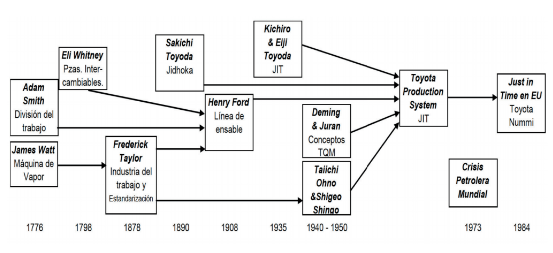
\includegraphics[scale=0.8]{images/historialean.png}
\caption{Linea temporal Lean Manufacturing \citep{socconini2019}}
\end{figure}

\subsection{Técnicas y herramientas Lean}

Las técnicas asociadas a Lean Manufacturing pueden implantarse de forma independiente o conjunta, atendiendo a las características específicas de cada caso. Su aplicación debe ser objeto de un diagnóstico previo que establezca la hoja de ruta idónea. Se debe señalar que el número de técnicas es muy elevado, por lo que se propone separarlas en tres grupos \citep{leansis2017}. 
El primero estaría formado por aquellas cuyas características, claridad y posibilidad real de implantación las hacen aplicables a cualquier casuística de empresa:

\begin{description}
\item \textbf{Las 5S:} Técnica utilizada para la mejora de las condiciones de trabajo de la empresa a través de un excelente orden, organización y limpieza en el puesto de trabajo. El acrónimo corresponde a las iniciales en japones de las cinco palabras que definen las herramientas, y cuya fonética empieza con ''S": Seiri, Seiton, Seiso, Seiketsu y Shitsuke, que significan, respectivamente: eliminar lo innecesario, ordenar, limpiar e inspeccionar, estandarizar y crear hábito.

\item \textbf{SMED:} Sistemas empleados para la disminución de los tiempos de preparación. Esta se logra estudiando detalladamente el proceso e incorporando cambios radicales en la máquina, utillaje, herramientas e incluso el propio producto, que disminuyan los tiempos de preparación. SMED hace uso de las técnicas de calidad
para resolución de problemas como el análisis de Pareto, las seis preguntas clásicas ¿Qué? – ¿Cómo? – ¿Dónde? – ¿Quién? – ¿Cuándo? y los respectivos ¿Por qué? 

\item \textbf{Estandarización:} Técnica que persigue la elaboración de instrucciones escritas o gráficas que muestren el mejor método para hacer las cosas. Las características que debe tener una correcta estandarización se pueden resumir en los cuatro principios siguientes:

\begin{enumerate}
\item Descripciones simples y claras de los mejores métodos para producir cosas.
\item Proceder de mejoras hechas con las mejoras técnicas y herramientas disponibles en cada caso.
\item Garantizar su cumplimiento.
\item Considerarlos siempre como puntos de partida para mejoras posteriores.
\end{enumerate}

\item \textbf{TPM:} Conjunto de múltiples acciones de mantenimiento productivo total que persigue eliminar las pérdidas por tiempos de parada de las máquinas. Para ello, el TPM se propone los siguientes cuatro objetivos:

\begin{enumerate}
\item Maximizar la eficacia del equipo
\item Desarrollar un sistema de mantenimiento productivo para toda la vida útil del equipo, que se inicie en el mismo momento del diseño de la máquina, y que incluirá a lo largo de toda su vida acciones de mantenimiento preventivo sistematizad y mejora de la mantenibilidad mediante reparaciones o modificaciones.
\item Implicar a todos los departamentos que planifican, diseñan, utilizan o mantienen los equipos.
\item Implicar activamente a todos los empleados, desde la alta dirección hasta los operarios, incluyendo mantenimiento autónomo de empleados y actividades en pequeños grupos.
\end{enumerate}

\item \textbf{Control Visual:} Conjunto de técnicas de control y comunicación visual que tienen por objetivo facilitar a todos los empleados el conocimiento del estado del sistema y del avance de las actividades de mejora. El control visual se focaliza exclusivamente en aquella información de alto valor añadido que ponga en evidencia las pérdidas en el sistema y las posibilidades de mejora. Hay que tener en cuenta que, en muchos casos, las fábricas usan estadísticas, gráficas y cifras de carácter estático y especializado que solo sirven a una pequeña parte de los responsables de la toma de decisión

\end{description}

El segundo grupo está conformado por aquellas técnicas que, aunque aplicables en cualquier situación, exigen un mayor compromiso y cambio cultural de todas las personas, tanto directivos, mandos intermedios y operarios:

\begin{description}
\item \textbf{Jidoka:} Técnica basada en la incorporación de sistemas y dispositivos que otorgan a las máquinas la capacidad de detectar que se están produciendo errores. Este proceso consta de 10 etapas:

\begin{itemize}
\item Autonomación del proceso: transferir esfuerzo del operario en el esfuerzo de la máquina.
\item Autonomación de sujetar: sustitución de apriete manual por sistemas accionados mecánicamente.
\item Autonomación de alimentación: Alimentación automática.
\item Autonomación de paradas:El sistema de alimentación para correctamente la máquina al final del proceso.
\item Autonomación de retornos: Finalizado y parado el proceso correctamente, el sistema retorna a la situación de inicio sin ayuda del operario.
\item Autonomación de retirada de piezas: Finalizado el proceso y retorno, la pieza es retirada automáticamente de forma que la siguiente pieza puede ser cargada sin necesidad de manipular la anterior.
\item Mecanismos a prueba de errores: Para prevenir la transferencia de piezas defectuosas al proceso siguiente,, se instalan dispositivos para detectar errores, parar la producción y alertar al operario.
\item Autonomación de carga: La pieza es cargada si necesidad del operario.
\item Autonomación de inicio: Completados los pasos anteriores, la máquina debe empezar a procesar piezas de forma autónoma.
\item Autonomación de transferencia: Se enlazan operaciones mediante sistemas de transferencia que eviten la intervención del operario.
\end{itemize}

\item \textbf{Técnicas de calidad:} Conjunto de técnicas proporcionadas por los sistemas de garantías de calidad que persiguen la disminución y eliminación de defectos. Para alcanzar estos objetivos, se propugna el uso intensivo de las técnicas de calidad, destacando entre todas ellas los chequeos de autocontrol, la Matriz de Autocalidad,

\end{description}

El último grupo está conformado por técnicas más específicas que cambian la forma de planificar, programar  y controlar los medios de producción y la cadena logística. 

\begin{description}
\item \textbf{Heijunka:} Conjunto de técnicas que sirven para planificar y nivelar la demanda de clientes, en volumen y variedad, durante un periodo de tiempo y que permiten a la evolución hacia la producción en flujo continuo, pieza a pieza.

\item \textbf{Kanban:} Sistema de control y programación sincronizada de la producción basado en tarjetas.
\end{description}


\section{Design Thinking}

\subsection{Metodologías ágiles}

\subsection{Design Thinking}

\subsection{Fases del Design Thinking}


\section{Herramientas de software}

\subsection{Lenguajes de programación orientada a objetos}

\subsection{Lenguajes de hojas de estilo}

\subsection{Bases de datos}

\subsection{Arquitectura Cliente-Servidor}

\subsection{API}

\subsection{Ordenadores de placa reducida}



 

% Figura: \'Arbol XML 1
%\begin{figure}[tp]
%  \centering
%  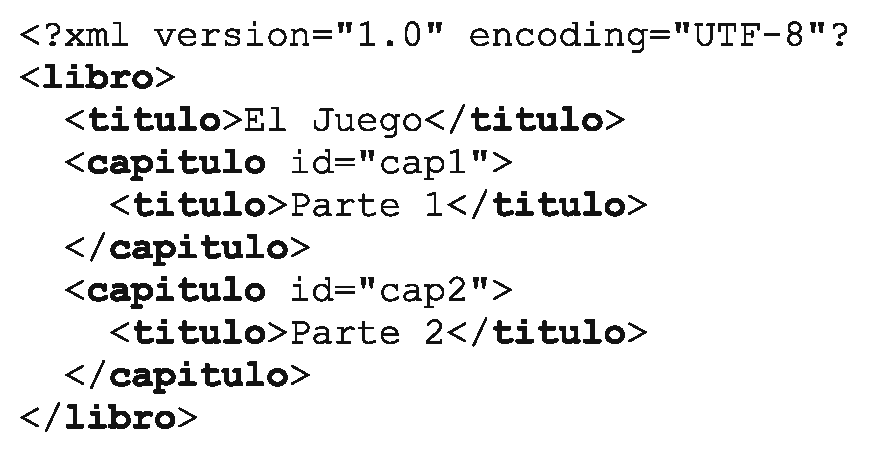
\includegraphics[scale=.5]{images/XML-document-example1}
%  \caption{\em Modelo de árbol para un documento XML.}
%  \label{fig:xml-tree-exa1}
%\end{figure}



